\chapter{Modello concettuale}\label{chp:modello-concettuale}
\begin{figure}[ht]
\centering
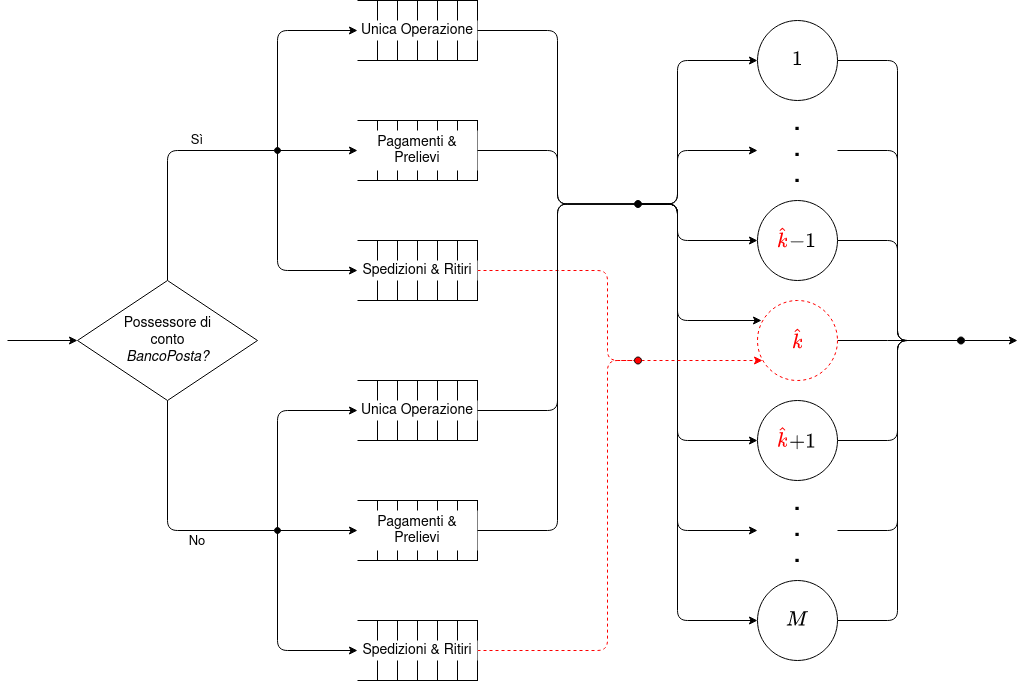
\includegraphics[width=\linewidth]{modello-concettuale-1}
\caption{Diagramma del sistema \textbf{Poste Italiane}}
\label{fig:modello-concettuale-1}
\end{figure}

Il funzionamento del sistema è illustrato dal diagramma in figura \ref{fig:modello-concettuale-1}. Di seguito è riportata una descrizione degli elementi in esso utilizzati:
\begin{itemize}
\item Il rombo rappresenta un meccanismo di ripartizione del flusso in ingresso nelle opportune code, a seconda della titolarità o meno di un conto \textsl{BancoPosta} da parte dei clienti.
\item Ciascuna coda modella una fila di clienti possessori dello stesso tipo di ticket.
\item Ciascun servente rappresenta uno sportello dell'ufficio postale
\begin{itemize}
\item Il $\ded$-esimo servente (evidenziato in {\color{red} rosso}) rappresenta lo sportello dedicato per la gestione dei ticket di tipo \sr{}, il cui comportamento è stato già illustrato nel flow chart in figura \ref{fig:presentazione-1}.
\end{itemize}
\end{itemize}

Ad ogni istante di tempo, lo stato del sistema è univocamente determinato dai valori assunti dalle seguenti variabili di stato:
\begin{itemize}
\item Per ciascuno sportello $i$ (con $i \in \lbrace 1, 2, \dots, \ded-1, \ded+1, \dots, M \rbrace$) si ha:
\begin{equation}
Server_i \in
\left\lbrace
\begin{array}{l l l}
\mathtt{IDLE}, & \mathtt{UNICA\_OP\_BP}, & \mathtt{PAGAM\_PREL\_BP},\\ 
\mathtt{UNICA\_OP\_STD}, & \mathtt{PAGAM\_PREL\_STD}
\end{array}
\right\rbrace
\end{equation}
\item Per lo sportello dedicato, ovvero il $\ded$-esimo in figura \ref{fig:modello-concettuale-1}, si ha:
\begin{equation}
Server_\ded \in 
\left\lbrace
\begin{array}{l l l}
\mathtt{IDLE}, & \mathtt{UNICA\_OP\_BP}, & \mathtt{PAGAM\_PREL\_BP},\\ 
\mathtt{UNICA\_OP\_STD}, & \mathtt{PAGAM\_PREL\_STD}, & \mathtt{SPED\_RIT\_BP},\\\mathtt{SPED\_RIT\_STD}
\end{array}
\right\rbrace
\end{equation}
\item Per ciascuna tipologia di ticket $(h, j)$ con:
\begin{itemize}
\item $h \in \lbrace \mathtt{BANCO\_POSTA},\ \mathtt{STANDARD}\rbrace$
\item $j \in \lbrace \mathtt{UNICA\_OP},\ \mathtt{PAGAM\_PREL},\ \mathtt{SPED\_RIT} \rbrace$
\end{itemize}
il livello di occupazione dei clienti è modellato dalla variabile $Customers_{h,j}$.
\end{itemize}

Infine, si assume che:
\begin{itemize}
\item I clienti abbiano un comportamento di tipo \textsl{one-step}\footnote{Avere un comportamento di tipo \textsl{one-step} significa che vi può essere lo spostamento di un solo cliente alla volta.}.
\item Non è possibile avere uno sportello libero se in coda è presente almeno un cliente con ticket processabile da tale sportello (sistema \textsl{work conserving}\footnote{La proprietà di \textsl{work conserving} è valida entro i vincoli imposti dal caso di studio.}).
\item All'inizio ed alla fine del periodo d'osservazione lo stato del sistema è il seguente:
\begin{equation}
\begin{cases}
Server_i =\mathtt{IDLE} & \forall\ i \in \lbrace 1, 2, \dots, M \rbrace \\[1em]
Customers_{h,j} = \mathtt{EMPTY} & \forall\ h \in \lbrace \mathtt{BANCO\_POSTA},\ \mathtt{STANDARD}\rbrace\ \wedge \\
& \forall\ j \in \lbrace \mathtt{UNICA\_OP},\ \mathtt{PAGAM\_PREL},\ \mathtt{SPED\_RIT} \rbrace
\end{cases}
\end{equation}
\end{itemize}


